\chapter{Dimensionering}

Figur \ref{fig:hej} viser de nye byggefelter inden for henholdsvis delområde A og delområde B til Strøybergs Palæ (\citep{lokalplan}, s. 16). Denne rapport fokuserer på byggefeltet inden for delområde B, hvor ny bebyggelse, ifølge lokalplan 1-1-107, må opføres i 3 etager samt en tagetage og med en kælder maksimalt 2 m over terræn. Ved opførsel af ny bebyggelse i delområde B, skal to nuværende mindre bygninger fjernes. 

\begin{figure}[htbp]
	\centering
	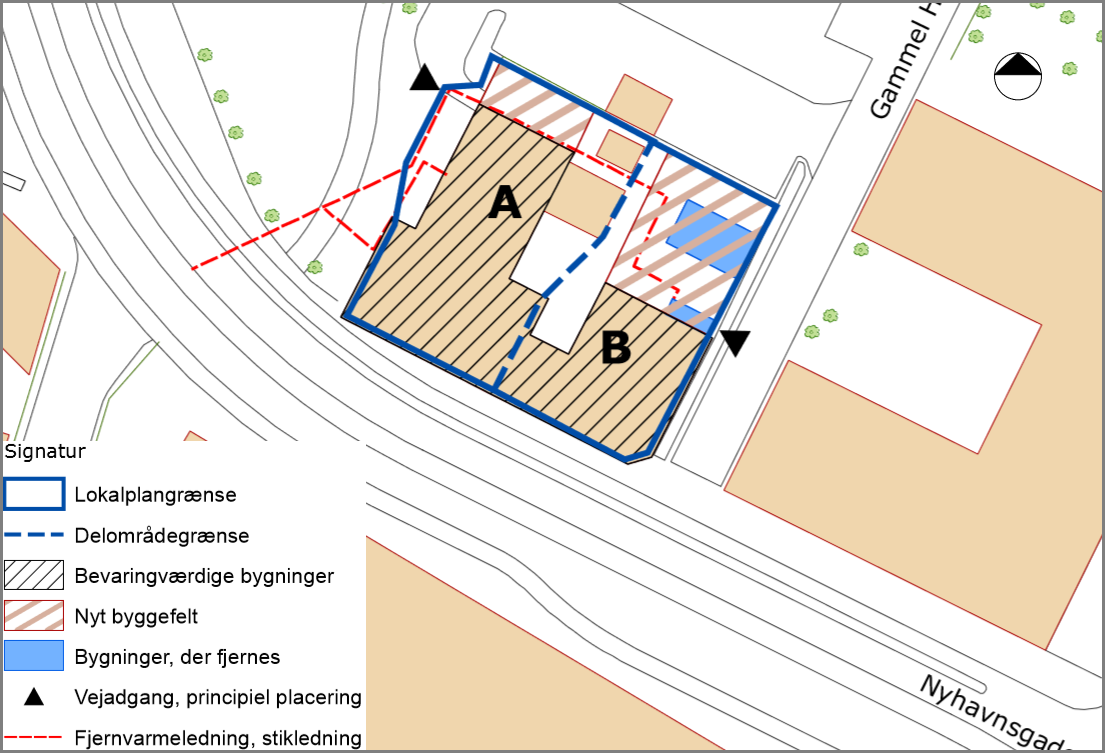
\includegraphics[width=0.7\textwidth]{billeder/signatur.png}
	\caption{Lokalplan 1-1-107, delområde A og B}
	\label{fig:hej}
\end{figure}

Med udgangspunkt i lokalplan 1-1-107 har bygningen fået de størrelser og dimensioner, som ses på Figur \ref{fig:farvel}.
\newline \indent{     }  Tilbygningen bliver 12,5 meter lang og 12 meter bred i henhold til den eksisterende bygningsbredde. Kælderen har en højde på i alt 3,25 m, hvor 1,25 m ligger over terræn. Stueetagen, 1. sal og 2. sal har hver især en højde på 4,9 m og tagetagen har en højde på 3 meter med en hældning på 26,6 grader. I alt er tilbygningen 19 m høj over terræn.

\begin{figure}[htbp]
	\centering
	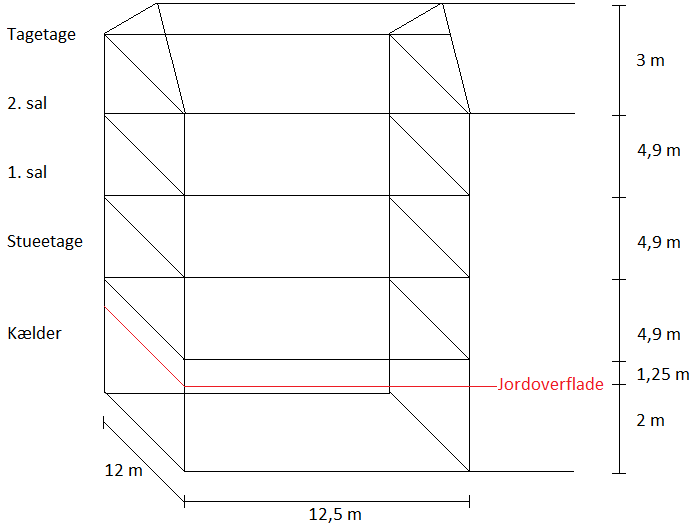
\includegraphics[width=0.7\textwidth]{billeder/tilbygning2.png}
	\caption{Tilbygningens dimensioner}
	\label{fig:farvel}
\end{figure}

For at kunne beregne de laster som påvirker tilbygningen, er der opstillet nedenstående statisk system for bygningen. Systemet er opstillet som en bjælkekonstruktion.
\newline
\newline
FIGURE HER!

\section{Laster}
Lidt tekst her.

\subsection{Permanent last}
Indsætte her.

\subsection{Variable laster}
Af variable laster optræder der både snelast og vindlast på bygningen, og disse udregnes efter Dansk Standard Eurocode 1991.

\subsubsection{Snelast}
Til at beregne hvordan snelasten påvirker tilbygningen anvendes den karaktiske snelast og formlen:
\begin{center}
$s=\mu_i\cdot C_e\cdot C_t \cdot s_k$
\end{center}
\begin{itemize}
	\item[-] $s$: karakteristisk snelast
	\item[-] $\mu_i$: formfaktoren for snelasten, som sættes til 0.8 (\citep{EU91}, tabel 5.2 s. 53)
	\item[-] $C_e$: eksponeringsfaktoren
	\item[-] $C_t$: termisk faktor, som sættes til 1.0 (\citep{EU91}, s. 52)
	\item[-] $s_k$: karakteristisk terrænværdi, som sættes til $1 \frac{kN}{m^2}$ (\citep{EU91}, s. 49)
\end{itemize}
Til at bestemme den karakteristiske snelast, beregnes eksponeringsfaktoren $C_e$.
\newline
\newline
Eksponeringsfaktoren, $C_e$, bestemmes ved:
\begin{center}
$C_e=C_{top}\cdot C_s$
\end{center}
\begin{itemize}
	\item[-] $C_{top}$: topografi faktor, som sættes til 1.0 (\citep{EU91}, tabel 5.1 s. 51)
	\item[-] $C_s$: størrelse faktor, som sættes til 1.0 (\citep{EU91}, s. 51-52)
\end{itemize}
Eksponeringsfaktoren kan nu bestemmes til:
\begin{center}
$C_e=1.0\cdot 1.0=1.0$
\end{center}
Strøybergs Palæ har et saddeltag, og dermed skal der tages højde for tre lasttilfælde, som ses på Figur INDSÆTTE FIGUR!
\newline
\newline
\underline{Lasttilfælde 1}
\begin{center}
$s_1=0.8\cdot 1.0\cdot 1.0\cdot 1 \frac{kN}{m^2}=0.8 \frac{kN}{m^2}$
\end{center}
\underline{Lasttilfælde 2 og 3}
\begin{center}
$s_2=\frac{1}{2}\cdot 0.8\cdot 1.0\cdot 1.0\cdot 1 \frac{kN}{m^2}=0.4 \frac{kN}{m^2}$
\end{center}
\underline{Lasttilfælde 4}
\begin{center}
	$s_4=\mu_w\cdot C_e\cdot C_t\cdot s_k \frac{kN}{m^2}$
\end{center}
\begin{itemize}
	\item[-] $\mu_w$: formfaktoren, som sættes til 1.2 eftersom $\alpha$ er $26.565^{\circ}$ (\citep{EU91}, s. 55)
\end{itemize}
Den karakteristiske snelast for lasttilfælde 4 kan nu bestemmes til:
\begin{center}
	$s_4=1.2\cdot 1.0\cdot 1.0\cdot 1 \frac{kN}{m^2}=1.2 \frac{kN}{m^2}$
\end{center}
I og med at lasttilfælde 4 giver den største last, anvendes denne til videre beregning.

\subsubsection{Vindlast}
Vindlasten beregnes for det højeste punkt på konstruktionen, hvilket er på tagspidsen for tilbygningen, da det er det punkt, hvor vinden er kraftigst.
\newline
\newline
FIGUR! - henvis til den med taget, som skal være i egenlasten
\newline
\newline
Til at bestemme vindlasten på tilbygningen bruges følgende formel:	
\begin{center} $w_e=q_p(z_e)$$\cdot$$c_{pe}$
\end{center}
\begin{itemize}
	\item[-] $q_p$: peakhastighedstrykket
	\item[-] $z_e$: referencehøjden for det udvendige vindtryk
	\item[-] $c_{pe}$: formfaktoren for det udvendige vindtryk
\end{itemize}
Den maksimale belastning fra vinden, peakhastighedstrykket $q_p$, bestemmes ved:
\begin{center}
$q_p(z_e)=[1+7I_v(z_e)]$$\cdot$$\frac{1}{2}$$\cdot$p$\cdot$$v_m^2(z_e)$
\end{center}
\begin{itemize}
	\item[-] $I_v$: vindturbulens
	\item[-] $\rho$: densiteten for luft $1.25 \frac{kg}{m^3}$
	\item[-] $v_m$: middelvindhastigheden
\end{itemize}
For at bestemme peakhastigheden, beregnes først vindturbulens $I_v(z)$ samt middelvindhastigheden $v_m$.
\newline
\newline
Vindturbulens, $I_v(z)$, bestemmes ved:
\begin{center}
$I_v(z)=\frac{\sigma_v}{V_m(z)}=\frac{k_1}{c_0(z)\cdot ln(\frac{z}{z_0})}$
\end{center}
\begin{itemize}
	\item[-] $k_1$: turbulensfaktor, sættes til 1.0 (\citep{EU91}, s. 82)
	\item[-] $c_0(z)$: orografifaktoren, som sættes til 1.0 (\citep{EU91}, s. 78)
	\item[-] $z$: højde, som er 19 m
	\item[-] $z_0$: ruhedslængde, som sættes til 1.0 for terrænkategori IV (\citep{EU91}, s. 79)
\end{itemize}
Vindturbulensen kan nu bestemmes til:
\begin{center}
$I_v(z)=\frac{1.0}{1.0\cdot ln(\frac{19}{1.0})}=0.340$
\end{center}
Middelvindhastigheden, $v_m$, bestemmes ved:
\begin{center}
$v_m(z)=c_r(z)\cdot c_0(z)\cdot v_b$
\end{center}
\begin{itemize}
	\item[-] $c_r(z)$: ruhedsfaktor
	\item[-] $v_b$: basisvindhastigheden
\end{itemize}
Til at bestemme middelvindhastigheden, beregnes basisvindhastigheden samt ruhedsfaktor.
\newline
\newline
Basisvindhastigheden, $v_b$, bestemmes ved:
\begin{center}
$v_b=c_{dir}\cdot c_{season}\cdot v_{b,0}$
\end{center}
\begin{itemize}
	\item[-] $c_{dir}$: retningsfaktor, som sættes til 1.0 (\citep{EU91}, tabel 1a s. 77)
	\item[-] $c_{season}$: årstidsfaktor, som sættes til 1.0 (\citep{EU91}, tabel 1b s. 77)
	\item[-] $v_{b,0}$: grundværdi for basisvindhastigheden, som sættes til 24 $\frac{m}{s}$, da dette er gældende for størstedelen af Danmark (\citep{EU91}, s. 77)
\end{itemize}
Basisvindhastigheden kan nu bestemmes til:
\begin{center}
$v_b=1.0\cdot 1.0\cdot 24 \frac{m}{s}=24 \frac{m}{s}$
\end{center}
Ruhedsfaktor, $c_r(z)$, bestemmes ved:
\begin{center}
$c_r(z)=k_r\cdot ln(\frac{z}{z_0})$
\end{center}
\begin{itemize}
	\item[-] $k_r$: terrænfaktor
\end{itemize}
Terrænfaktoren, $k_r$, bestemmes ved:
\begin{center}
$k_r=0.19\cdot (\frac{z_0}{z_{0,II}})^{0.07}$
\end{center}
\begin{itemize}
	\item[-] $z_{0,II}$: værdi for ruhedslængde for terrænkategori II, som sættes til 0.05 (\citep{EU91}, s. 78-79)
\end{itemize}
\begin{center}
$k_r=0.19\cdot (\frac{1.0}{z_{0.05}})^{0.07}=0.234$
\end{center}
Ruhedsfaktor kan nu bestemmes til:
\begin{center}
$c_r(z)=0.234\cdot ln(\frac{19}{1.0})=0.690$
\end{center}
Middelvindhastigheden kan nu bestemmes til:
\begin{center}
$v_m(z)=0.690\cdot 1.0\cdot 24 \frac{m}{s}=16.569 \frac{m}{s}$
\end{center}
Peakhastighedstrykket $q_p$ i højden z, kan nu bestemmes til:
\begin{center}
$q_p(z_e)=[1+7\cdot 0.340]\cdot \frac{1}{2}\cdot 1.25 \frac{kg}{m^3}\cdot (16.569 \frac{m}{s})^2=0.579 \frac{kN}{m^2}$
\end{center}

HVAD GØR VI NU??

\begin{figure}[htbp]
	\centering
	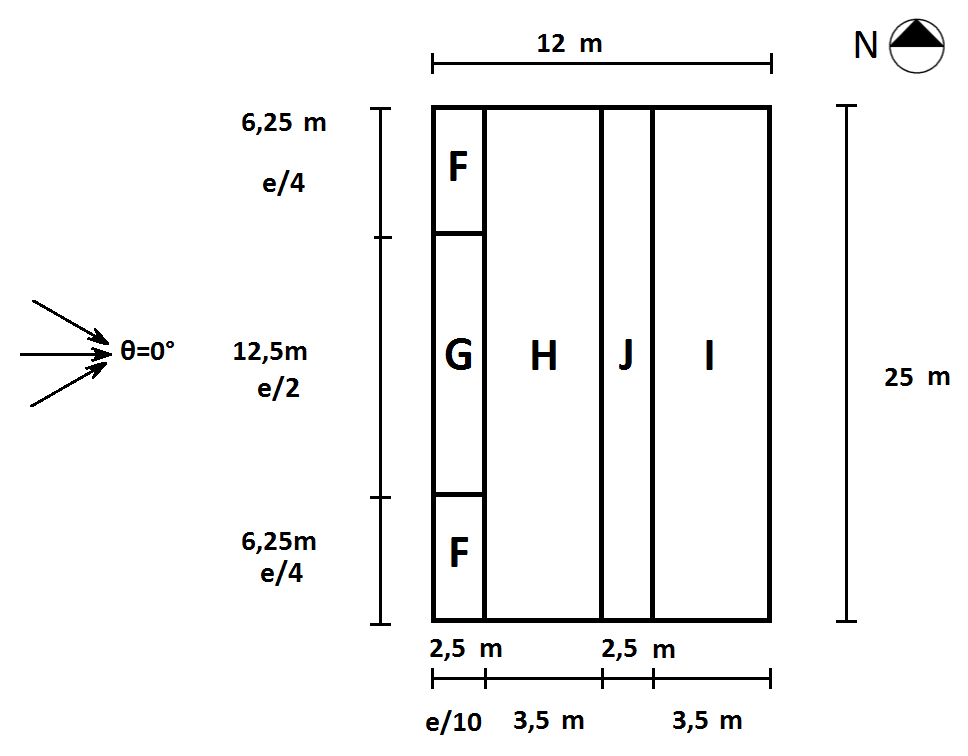
\includegraphics[width=0.5\textwidth]{billeder/opdeling.png}
	\caption{Zoneinddeling af taget}
	\label{fig:tag}
\end{figure}

For alle zoner bestemmes $c_{pe,10}$. Der opstilles en lineær ligning med sammenhæng mellem $c_{pe,10}$ værdierne og graderne 15 og 30. Herefter indsættes taghældningen, $26.565^{\circ}$ i ligningen og værdien for $c_{pe,10}$ i den pågældende zone fås.
\newline
\newline
\underline{Zone F}
\newline
Ud fra tabel 7.4a (\citep{EU91}, s. 112) er de negative værdier for zone F -0.9 og -0.5. Her ud fra fås ligningen, og $c_{pe,10,neg}$ bestemmes:
\begin{center}
	$f(\alpha)=0.0267\cdot \alpha - 1.3 \to c_{pe,10,neg}=-0.592$
\end{center}
De positive værdier for zone F er: 0.2 og 0.7. Her ud fra fås ligningen, og $c_{pe,10,pos}$ bestemmes:
\begin{center}
	$f(\alpha)=0.0333\cdot \alpha - 0.3 \to c_{pe,10,pos}=0.585$
\end{center}

\underline{Zone G}
\newline
De negative værdier for zone G er: -0.8 og -0.5. Her ud fra fås ligningen, og $c_{pe,10,neg}$ bestemmes:
\begin{center}
	$f(\alpha)=0.02\cdot \alpha - 1.1 \to c_{pe,10,neg}=-0.569$
\end{center}
De positive værdier for zone G er: 0.2 og 0.7. Her ud fra fås ligningen, og $c_{pe,10,pos}$ bestemmes:
\begin{center}
	$f(\alpha)=0.0333\cdot \alpha - 0.3 \to c_{pe,10,pos}=0.585$
\end{center}

\underline{Zone H}
\newline
De negative værdier for zone H er: -0.3 og -0.2. Her ud fra fås ligningen, og $c_{pe,10,neg}$ bestemmes:
\begin{center}
	$f(\alpha)=0.00667\cdot \alpha - 0.4 \to c_{pe,10,neg}=-0.223$
\end{center}
De positive værdier for zone H er: 0.2 og 0.4. Her ud fra fås ligningen, og $c_{pe,10,pos}$ bestemmes:
\begin{center}
	$f(\alpha)=0.0133\cdot \alpha - 1.178\cdot 10^{-16} \to c_{pe,10,pos}=0.354$
\end{center}

\underline{Zone I}
\newline
Den negative værdi for zone I er: -0.4. Her ud fra fås ligningen, og $c_{pe,10,neg}$ bestemmes:
\begin{center}
	$f(\alpha)=-5.234\cdot 10^{-18}\cdot \alpha - 0.4 \to c_{pe,10,neg}=-0.4$
\end{center}
Den positive værdi for zone I er: 0.0. Her ud fra fås ligningen, og $c_{pe,10,pos}$ bestemmes:
\begin{center}
	$f(\alpha)=0.0 \to c_{pe,10,pos}=0.0$
\end{center}

\underline{Zone J}
\newline
De negative værdier for zone J er: -1.0 og -0.5. Her ud fra fås ligningen, og $c_{pe,10,neg}$ bestemmes:
\begin{center}
	$f(\alpha)=0.0333\cdot \alpha - 1.5 \to c_{pe,10,neg}=-0.615$
\end{center}
Den positive værdi for zone J er: 0.0. Her ud fra fås ligningen, og $c_{pe,10,pos}$ bestemmes:
\begin{center}
	$f(\alpha)=0.0 \to c_{pe,10,pos}=0.0$
\end{center}
INDSÆTTE DET SIDSTE!

\section{Lastkombinationer}
INTROTEKST
\newline
\newline
\underline{Egenlast}
\newline
INDSÆTTE!